\documentclass[12pt]{article}
\usepackage{graphicx}\usepackage{hyperref}\usepackage{natbib}
\graphicspath{ {../figures/} }

\title{REMARK \LaTeX{} Template}
\author{Econ-ARK Team}
\date{\today}

\bibliographystyle{plainnat}

\begin{document}
\maketitle

\begin{abstract}
The \href{https://github.com/econ-ark/REMARK}{REMARK} infrastructure permits the construction of reproducible scientific computing results, along with associated documentation.
\end{abstract}

\section{Introduction}

\cite{carroll_et_al-proc-scipy-2018} describe plans for the \href{https://econ-ark.org}{Econ-ARK} toolkit, among which is the development of an infrastructure that will allow for the construction of \href{https://econ-ark.org/materials/REMARK}{REMARK} repositories whose aim is to make it easy to construct reproducible scientific computational results.

\section{Other Parts of the Toolkit}

The chief component of the toolkit is the \href{https://github.com/econ-ark/HARK}{HARK} set of tools for solving heterogeneous agent models, particularly of consumption and other financial choices.

Here are some examples produced by the toolkit:

\begin{figure}
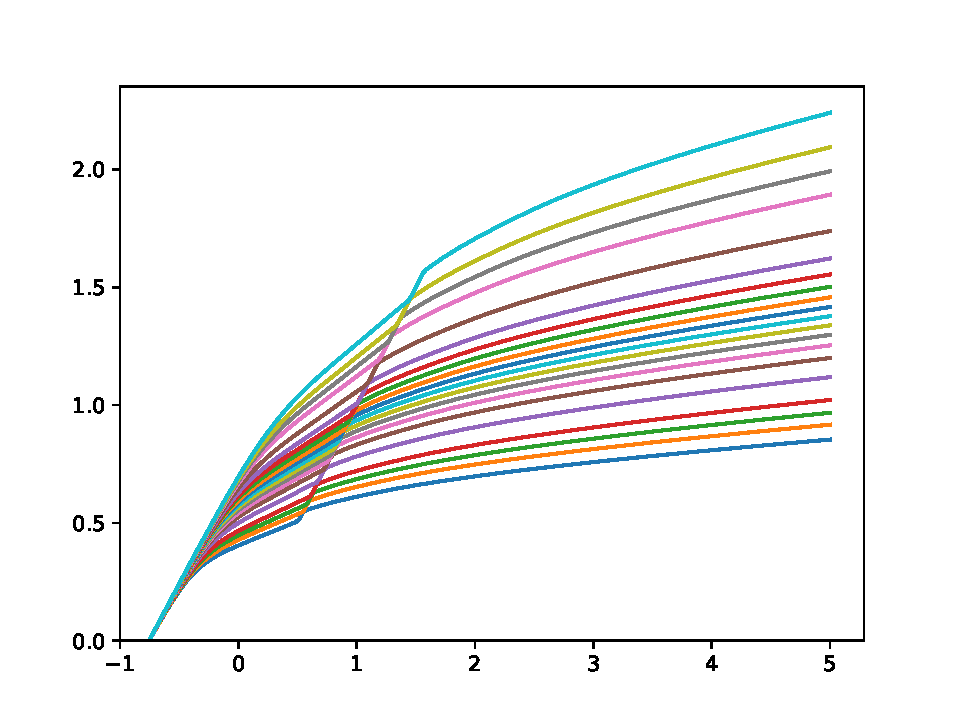
\includegraphics[scale=0.8]{cFunc}
\end{figure}
\begin{figure}
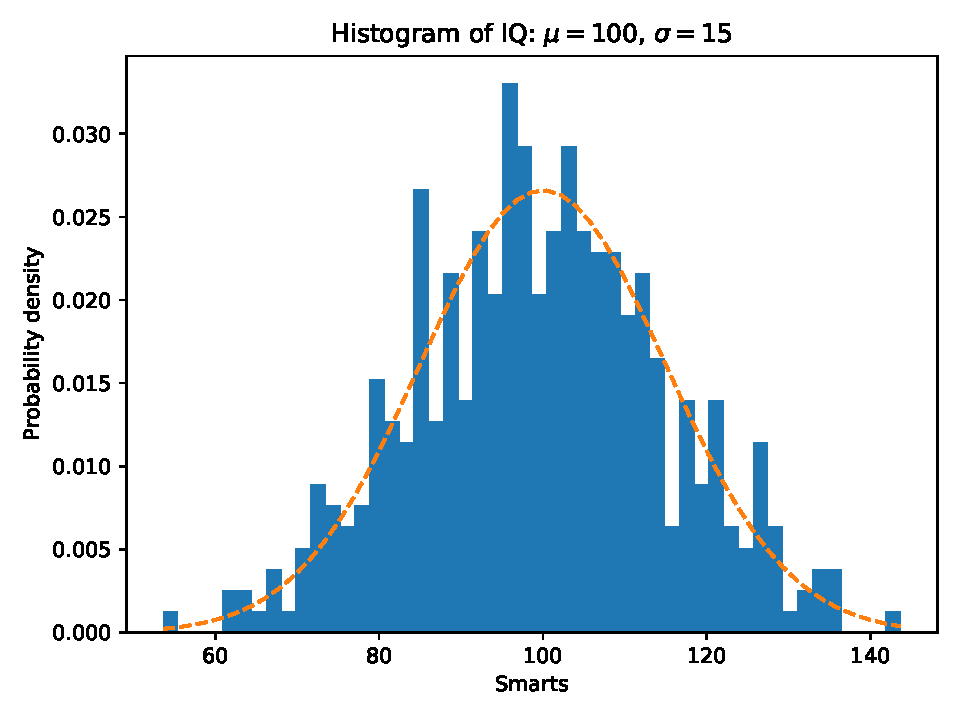
\includegraphics[scale=0.8]{dist}
\end{figure}

\bibliography{./latex/REMARK-starter-example}

\end{document}

